%% ============================================================
%%  First Review Report - FYP
%%  Physics-Informed Gait Modeling for Freezing-of-Gait Detection
%%  Department of Instrumentation and Control Engineering
%%  National Institute of Technology Tiruchirappalli
%% ============================================================
%%
%%  OVERLEAF INSTRUCTIONS
%%  1. Create a new Overleaf project and upload this as main.tex
%%  2. Set Compiler to pdfLaTeX (Menu -> Compiler -> pdfLaTeX)
%%  3. Logo: upload NITT_Logo.png and replace the \fbox{...} block
%%     in the header with: \includegraphics[height=1.8cm]{NITT_Logo.png}
%% ============================================================

\documentclass[12pt,a4paper]{article}

%% ---- Packages ----
\usepackage[a4paper, top=3.8cm, bottom=2.5cm, left=2.5cm, right=2.5cm]{geometry}
\usepackage{graphicx}
\usepackage{amsmath,amssymb}
\usepackage{fancyhdr}
\usepackage{titlesec}
\usepackage{booktabs}
\usepackage{array}
\usepackage{multirow}
\usepackage{enumitem}
\usepackage{setspace}
\usepackage{parskip}
\usepackage{xcolor}
\usepackage{cite}
\usepackage{adjustbox}
\usepackage[hidelinks,colorlinks=true,linkcolor=black,urlcolor=blue,citecolor=black]{hyperref}

%% ---- TikZ & PGFPlots ----
\usepackage{tikz}
\usepackage{pgfplots}
\pgfplotsset{compat=1.18}
\usetikzlibrary{shapes.geometric,arrows.meta,positioning,fit,
                decorations.pathreplacing,calc,patterns,backgrounds}

%% ---- Colours ----
\definecolor{blockblue}{RGB}{52,101,164}
\definecolor{blockorange}{RGB}{206,92,0}
\definecolor{blockgreen}{RGB}{78,153,78}
\definecolor{blockgray}{RGB}{120,120,120}
\definecolor{lightblue}{RGB}{220,234,255}
\definecolor{lightorange}{RGB}{255,238,210}
\definecolor{lightgreen}{RGB}{220,245,220}
\definecolor{lightgray}{RGB}{240,240,240}

%% ================================================================
%%  HEADER
%% ================================================================
\pagestyle{fancy}
\fancyhf{}
\fancyhead[C]{%
  \begin{tabular}{@{}l@{}}
    \begin{tabular}{@{}l@{\hspace{0.6em}}c@{}}
      \raisebox{-0.3\height}{%
        \includegraphics[height=1.8cm]{NITT Logo.png} 
      }
      &
      \begin{tabular}[c]{@{}c@{}}
        \textbf{Department of Instrumentation and Control Engineering}\\[4pt]
        \textbf{National Institute of Technology Tiruchirappalli}
      \end{tabular}
    \end{tabular}\\[4pt]
    \rule{\textwidth}{0.4pt}
  \end{tabular}%
}
\fancyfoot[C]{\thepage}
\renewcommand{\headrulewidth}{0pt}
\setlength{\headheight}{52pt}
\addtolength{\topmargin}{-20pt}

%% ---- Section formatting ----
\titleformat{\section}{\large\bfseries}{}{0em}{}[\titlerule]
\titleformat{\subsection}{\normalsize\bfseries}{}{0em}{}
\titleformat{\subsubsection}{\normalsize\bfseries\itshape}{}{0em}{}

%% ================================================================
\begin{document}

%% ================================================================
%%  COVER PAGE
%% ================================================================
\thispagestyle{fancy}
\vspace*{1.5cm}

\begin{center}
  {\LARGE\textbf{\underline{First Review Report}}}

  \vspace{1.2cm}
  \begin{minipage}{0.85\textwidth}
    \begin{flushleft}
      {\large\textbf{\underline{Title:}}}\\[6pt]
      \hspace{1em}\parbox{0.9\linewidth}{Physics-Informed Gait Modeling for Freezing-of-Gait
        Detection in Parkinson's Disease Using Wearable Sensors}
    \end{flushleft}
  \end{minipage}

  \vspace{1.0cm}
  \begin{minipage}{0.85\textwidth}
    \begin{flushleft}
      {\large\textbf{\underline{Guide's Name:}} Dr. D. Ezhilarasi}\\[6pt]
      \hspace{1em}% Insert guide name here
    \end{flushleft}
  \end{minipage}

  \vspace{1.0cm}
  \begin{minipage}{0.85\textwidth}
    \begin{flushleft}
      {\large\textbf{\underline{Team Members:}}}
    \end{flushleft}
  \end{minipage}

  \vspace{0.5cm}
  \begin{tabular}{|p{3.8cm}|p{5cm}|p{5cm}|}
    \hline
    \textbf{Roll No} & \textbf{Name} & \textbf{Signature} \\
    \hline 
    & & \\[2.2cm]
    \hline
  \end{tabular}
\end{center}

%% ================================================================
%%  PAGE 2 -- OBJECTIVES
%% ================================================================
\newpage
\section*{Objectives}

\begin{itemize}[leftmargin=*, itemsep=6pt]
  \item Develop a physics-informed latent Neural ODE model of human gait, enforcing smoothness,
        periodicity (limit-cycle behaviour), and monotonic phase progression in the latent dynamics.
  \item Reframe Freezing of Gait (FoG) detection as identification of breaks or anomalies in these
        latent gait dynamics, rather than simple time-series classification.
  \item Train the model on wearable inertial (accelerometer) gait data from the public Daphnet
        dataset so that normal walking maps to a regular 2-D limit-cycle in latent space,
        requiring \textbf{no labelled FoG data} for training.
  \item Detect FoG episodes by monitoring the dynamics residual
        $\bigl(r(t)=\lvert\dot{z}(t)-f_\theta(z(t))\rvert\bigr)$ and latent phase stagnation
        $\bigl(\phi'(t)\approx 0\bigr)$ --- producing \textbf{clinically interpretable biomarkers}
        (spikes in $r(t)$ or plateaus in $\phi(t)$) that explain \emph{why} a window is flagged.
  \item Conduct a \textbf{multi-paradigm comparison} of three detection approaches --- supervised
        classification (1D-CNN, CNN--LSTM), unsupervised anomaly detection (Convolutional
        Autoencoder, One-Class SVM), and the proposed physics-informed anomaly detection --- under
        an identical LOSO evaluation protocol.
\end{itemize}

%% ================================================================
%%  PAGE 3 -- INTRODUCTION AND LITERATURE REVIEW
%% ================================================================
\newpage
\section*{Introduction and Literature Review}

Parkinson's Disease (PD) is a common progressive neurodegenerative movement disorder, affecting
roughly 1--5\% of people over age 60 and rising sharply with age \cite{techniques2023,ankle2025}.
One of its most debilitating motor symptoms is Freezing of Gait (FoG) --- typically defined as a
``brief, episodic absence or marked reduction of forward progression of the feet despite the intention
to walk'' \cite{techniques2023}. Patients often describe FoG as feeling ``glued to the floor,'' and
it occurs especially during gait initiation, turning, or navigating confined spaces
\cite{techniques2023,ankle2025}. FoG is frequent and disabling: roughly half of PD patients
experience freezing, and it affects nearly all advanced-stage patients. The episodic halts frequently
result in falls and injuries, severely impairing mobility and quality of life
\cite{techniques2023,deep2024}.

Because FoG is intermittent and unpredictable, accurate clinical assessment is inherently limited.
This has spurred strong interest in wearable sensor-based detection during everyday activities.
Inertial measurement units (IMUs) worn on the body can capture gait kinematics continuously and
non-invasively. Machine learning models trained on these signals can distinguish normal walking from
freezing episodes, enabling real-time assistive cueing and objective longitudinal monitoring.

The vast majority of prior work treats FoG detection as a standard supervised classification problem
on time-series data \cite{ankle2025,deep2024}. Brederecke (2023) trained a simple 1-D convolutional
network on wrist accelerometer data \cite{brederecke2023}. Pav\'{o}n et al.\ (2020) report
CNN--LSTM models achieving AUCs of approximately 0.92--0.94 \cite{pavon2020}. A recent
semi-free-living study with ankle-mounted accelerometers found a LOSO AUROC of approximately 0.93
\cite{ankle2025}, demonstrating that temporal patterns in IMU signals are genuinely predictive of
freezing.

However, data-driven classifiers carry important limitations. Sigcha et al.\ (2024) found that while
deep models may reach AUC~$\approx$~0.9 on the training dataset, performance on an unseen dataset
falls to AUC~$\approx$~0.65--0.84 \cite{deep2024}, suggesting overfitting to dataset-specific
artefacts. These models also offer little clinical interpretability.

A key mechanistic insight motivates our approach: normal human gait is fundamentally rhythmic and
cyclic \cite{gaitrhythm2008}. Plotnik et al.\ showed that PD patients with FoG have significantly
reduced gait rhythmicity and disrupted interlimb coupling \cite{gaitrhythm2008}. FoG is therefore
better characterised as a \emph{dynamical anomaly} --- a momentary collapse of the gait oscillator.

To embed this knowledge, we leverage Physics-Informed Neural Networks (PINNs)
\cite{raissi2019,mathworks2025}, which are trained to simultaneously fit data and satisfy known
physical constraints (ODEs/PDEs) \cite{raissi2019}. We frame gait as a 2-D autonomous latent system
governed by a Neural ODE \cite{chen2018}, enforcing smoothness, periodicity, and monotonic phase
via soft loss penalties. FoG is then detected as deviations from the learned limit cycle. To our
knowledge, this combination is novel in the FoG detection literature.

%% ================================================================
%%  PAGE 4+ -- DETAILED METHODOLOGY AND WORK COMPLETED
%% ================================================================
\newpage
\section*{Detailed Methodology and Work Completed}

\subsection*{System Overview}

The proposed system evaluates FoG detection across three distinct paradigms operating on the same
preprocessed IMU data.

\textbf{(i) Supervised classifiers} (1D-CNN and CNN--LSTM) map fixed-length IMU windows directly
to a FoG probability, using labelled normal \emph{and} FoG data for training. These represent the
performance ceiling when annotated data is available.

\textbf{(ii) Unsupervised anomaly detectors} (Convolutional Autoencoder and One-Class SVM) train
exclusively on normal-gait windows and flag reconstructions with high error or outlier scores as
FoG. These serve as paradigm-matched baselines for the PINN, isolating the contribution of
physics-informed constraints versus generic anomaly detection.

\textbf{(iii) The physics-informed branch} (PINN) also trains on normal-gait windows only, but
learns an explicit continuous dynamical law of healthy gait via a latent Neural ODE. At inference,
deviations from this law --- dynamics residuals and phase stagnation --- serve as interpretable
anomaly scores.

%% ---------------------------------------------------------------
%% FIGURE 1: System Architecture
%%
%% FIXES APPLIED:
%%   (1) Box style renamed 'sysbox' -- 'box' and 'step' are both reserved TikZ keys.
%%   (2) Brace node labels use 'text width + align=center' with NO '\\' in node text.
%%       Using '\\' inside a TikZ node without align=center triggers "Not allowed in LR mode".
%%   (3) All figures wrapped in \adjustbox{max width=\textwidth} to prevent margin overflow.
%% ---------------------------------------------------------------
\begin{figure}[ht]
\centering
\begin{adjustbox}{max width=\textwidth}
\begin{tikzpicture}[
  sysbox/.style={draw, rounded corners=3pt, minimum width=2.1cm, minimum height=0.7cm,
                 align=center, font=\small},
  bluebox/.style={sysbox, fill=lightblue,   draw=blockblue,   text=blockblue},
  orangebox/.style={sysbox, fill=lightorange, draw=blockorange, text=blockorange},
  greenbox/.style={sysbox, fill=lightgreen,  draw=blockgreen,  text=blockgreen},
  graybox/.style={sysbox,  fill=lightgray,   draw=blockgray},
  arr/.style={-{Stealth[length=5pt]}, thick},
  node distance=0.45cm and 0.6cm
]

\node[graybox, minimum width=1.8cm] (raw) {Raw IMU\\(9-ch, 64\,Hz)};
\node[graybox, right=0.7cm of raw, minimum width=2.0cm] (pre) {Preprocess\\(Filter, Window)};
\draw[arr] (raw) -- (pre);

%% Blue branch nodes
\node[bluebox, above right=0.55cm and 1.2cm of pre] (cnn)    {1D-CNN};
\node[bluebox, right=0.55cm of cnn]                 (cnncls) {FoG Prob.\\(sigmoid)};

\node[bluebox, below=0.55cm of cnn]  (lstm)    {CNN--LSTM};
\node[bluebox, right=0.55cm of lstm] (lstmcls) {FoG Prob.\\(sigmoid)};

%% Orange / PINN branch nodes
\node[orangebox, below=0.35cm of lstm] (enc) {Encoder\\$E_\phi$};
\node[orangebox, right=0.5cm of enc]   (ode) {Neural ODE\\$f_\theta$};
\node[orangebox, right=0.5cm of ode]   (dec) {Decoder\\$D_\psi$};
\node[greenbox,  right=0.5cm of dec]   (det) {Anomaly\\Score $r(t),\Delta\Phi$};

%% Shared vertical bus from Preprocess to all three branches
\coordinate (bus) at ($(pre.east) + (0.5,0)$);
\draw[arr] (pre.east) -- (bus);
\draw[arr] (bus) |- (cnn.west);
\draw[arr] (bus) |- (lstm.west);
\draw[arr] (bus) |- (enc.west);

%% Internal arrows
\draw[arr] (cnn)  -- (cnncls);
\draw[arr] (lstm) -- (lstmcls);
\draw[arr] (enc)  -- (ode);
\draw[arr] (ode)  -- (dec);
\draw[arr] (dec)  -- (det);

%% Decision box — vertically centred between cnncls and lstmcls
\node[greenbox, right=1.2cm of cnncls, yshift=-0.55cm] (decision)
  {\textbf{FoG / Normal} decision};

%% Shared vertical merge bus feeding into decision from the left
\coordinate (merge) at ($(decision.west) + (-0.35, 0)$);
\draw[arr] (cnncls.east)  -- ++(0.15,0) |- (merge) -- (decision.west);
\draw[arr] (lstmcls.east) -- ++(0.15,0) |- (merge);

%% Anomaly score enters decision from the right / below
\draw[arr] (det.east) -- ++(0.3,0) |- (decision.east);

%% Brace: Supervised Baselines (no mirror, top->bottom, opens right toward nodes)
\draw[decorate, decoration={brace, amplitude=5pt}, blockblue, thick]
  ([xshift=-8pt, yshift= 4pt]cnn.north west) --
  ([xshift=-8pt, yshift=-4pt]lstm.south west)
  node[midway, left=6pt, text width=1.5cm, align=center,
       font=\scriptsize\bfseries\color{blockblue}] {Supervised Baselines};

%% Brace: PINN Branch (no mirror, top->bottom, opens right toward nodes)
\draw[decorate, decoration={brace, amplitude=5pt}, blockorange, thick]
  ([xshift=-8pt, yshift= 4pt]enc.north west) --
  ([xshift=-8pt, yshift=-4pt]enc.south west)
  node[midway, left=6pt, text width=1.2cm, align=center,
       font=\scriptsize\bfseries\color{blockorange}] {PINN Branch};

\end{tikzpicture}
\end{adjustbox}
\caption{High-level system architecture. Both branches operate on identical preprocessed
         windows (3.2\,s, 40\,Hz, 75\% overlap). The supervised baselines (blue) output a
         direct FoG probability; the PINN branch (orange) detects FoG via anomaly scores
         derived from latent dynamics.}
\label{fig:system}
\end{figure}

Both branches share the same preprocessing and evaluation protocol: 3.2-second sliding windows at
40\,Hz with 75\% overlap, and Leave-One-Subject-Out (LOSO) cross-validation across all 10 subjects.

%% ---------------------------------------------------------------
\subsection*{Daphnet Freezing-of-Gait Dataset}

We use the Daphnet FoG dataset \cite{daphnet2023}, the most widely cited publicly available IMU
dataset for PD gait research. It contains recordings from 10 individuals with clinically confirmed
PD (8 of whom produced annotated FoG episodes), collected in a controlled laboratory setting.
Participants performed structured walking tasks designed to provoke FoG: corridor walking with turns,
navigation through narrow gaps, and stopping tasks. Each participant wore six tri-axial MEMS
accelerometers on both ankles (shanks), both thighs, and the lower back (trunk). We select 9 channels
from one ankle, one thigh, and the trunk \cite{ankle2025,pavon2020}. Labels per sample: 0 = normal,
1 = no-freeze trial (discarded), 2 = confirmed FoG. The dataset contains 237 annotated FoG episodes,
with approximately 10\% FoG samples overall.

\begin{table}[ht]
\centering
\caption{Daphnet dataset statistics after preprocessing (40\,Hz, 9-channel, 128-sample windows).}
\label{tab:dataset}
\renewcommand{\arraystretch}{1.3}
\begin{adjustbox}{max width=\textwidth}
\begin{tabular}{lcccc}
\toprule
\textbf{Property} & \textbf{Value} & & \textbf{Property} & \textbf{Value} \\
\midrule
Total subjects          & 10         & & Sampling rate (raw)  & 64\,Hz \\
Subjects with FoG       & 8          & & Sampling rate (used) & 40\,Hz \\
FoG episodes            & 237        & & Window length        & 3.2\,s (128 samples) \\
Approx.\ FoG proportion & $\sim$10\% & & Window stride        & 0.8\,s (75\% overlap) \\
IMU sensors used        & 3 (ankle, thigh, trunk) & & Channels per window & $128\times9$ \\
FoG episode duration    & 0.5--30\,s & & Class ratio (N:FoG)  & $\approx$9:1 \\
\bottomrule
\end{tabular}
\end{adjustbox}
\end{table}

%% ---------------------------------------------------------------
\subsection*{Data Preprocessing Pipeline}

A carefully designed preprocessing pipeline is essential to extract clean, consistent gait features.
Our pipeline, implemented in Python with \texttt{scipy}, \texttt{numpy}, and \texttt{pandas},
consists of seven sequential steps illustrated in Figure~\ref{fig:pipeline}.

%% ---------------------------------------------------------------
%% FIGURE 2: Preprocessing Pipeline
%% FIX: style named 'pipenode' -- avoids reserved TikZ key 'step'.
%% Multi-line node labels use \\ only inside nodes that have align=center (safe here).
%% ---------------------------------------------------------------
\begin{figure}[ht]
\centering
\begin{tikzpicture}[
  pipenode/.style={draw=blockblue, fill=lightblue, rounded corners=4pt,
                   minimum width=2.8cm, minimum height=0.65cm,
                   align=center, font=\small, text=blockblue},
  pipenote/.style={font=\scriptsize, text=blockgray, align=left},
  arr/.style={-{Stealth[length=5pt]}, thick, blockblue},
  node distance=0.38cm
]
\node[pipenode] (s1) {1.\ Label filtering};
\node[pipenode, below=of s1] (s2) {2.\ Resampling 64$\to$40\,Hz};
\node[pipenode, below=of s2] (s3) {3.\ Band-pass filter 0.3--15\,Hz};
\node[pipenode, below=of s3] (s4) {4.\ Axis alignment};
\node[pipenode, below=of s4] (s5) {5.\ Sliding window $N=128$, 75\% overlap};
\node[pipenode, below=of s5] (s6) {6.\ Window labelling: $>$50\% FoG $\Rightarrow$ FoG};
\node[pipenode, below=of s6] (s7) {7.\ $z$-score normalisation (per LOSO fold)};

\foreach \i/\j in {s1/s2,s2/s3,s3/s4,s4/s5,s5/s6,s6/s7}
  \draw[arr] (\i) -- (\j);

\node[pipenote, right=0.7cm of s1] {Remove label-1 (unreliable) samples};
\node[pipenote, right=0.7cm of s2] {Anti-alias LPF (8th-order Butterworth, 20\,Hz)};
\node[pipenote, right=0.7cm of s3] {Zero-phase \texttt{filtfilt}; remove drift \& noise};
\node[pipenote, right=0.7cm of s4] {Common frame: $x$=forward, $y$=vertical, $z$=lateral};
\node[pipenote, right=0.7cm of s5] {3.2\,s span $\geq$ 2 gait cycles; 0.8\,s latency};
\node[pipenote, right=0.7cm of s6] {Ambiguous 10--50\% windows discarded};
\node[pipenote, right=0.7cm of s7] {Prevent cross-subject data leakage};
\end{tikzpicture}
\caption{Sequential data preprocessing pipeline. Each step is applied to all 9 channels
         independently. LOSO-fold statistics are computed only on the training portion.}
\label{fig:pipeline}
\end{figure}

\begin{enumerate}[leftmargin=*, label=\textbf{Step \arabic*.}, itemsep=4pt]
  \item \textbf{Label filtering.} Samples labelled 1 are removed; only labels 0 (normal) and
        2 (FoG) are retained.
  \item \textbf{Resampling.} 64\,Hz $\to$ 40\,Hz with 8th-order anti-alias Butterworth LPF
        at 20\,Hz prior to decimation.
  \item \textbf{Band-pass filtering.} 4th-order zero-phase Butterworth, 0.3--15\,Hz, applied
        per channel via \texttt{scipy.signal.filtfilt} to avoid phase distortion \cite{ankle2025}.
  \item \textbf{Axis alignment.} IMU frames remapped to $x$=anteroposterior, $y$=vertical,
        $z$=mediolateral \cite{daphnet2023}.
  \item \textbf{Sliding-window segmentation.} $N=128$ samples (3.2\,s), stride 32 samples
        (0.8\,s, 75\% overlap).
  \item \textbf{Window labelling.} FoG if $>$50\% of samples are label 2; normal if $<$10\%;
        otherwise discarded, following Pav\'{o}n et al.\ \cite{pavon2020}.
  \item \textbf{Channel-wise normalisation.} Zero mean, unit variance per channel, computed on
        the training fold only to prevent data leakage.
\end{enumerate}

%% ---------------------------------------------------------------
\subsection*{Class Imbalance and Data Augmentation}

The dataset is approximately 90\% normal and 10\% FoG windows. We address this with two strategies
applied to the supervised baselines.

\textbf{Inverse-frequency loss weighting.}
\[
  w_{\mathrm{FoG}} = \frac{N_{\mathrm{normal}}}{N_{\mathrm{FoG}}}, \qquad w_{\mathrm{normal}} = 1.
\]
This ensures equal aggregate gradient contribution from both classes.

\textbf{Window-level oversampling with temporal jitter.} Each FoG training window is duplicated
twice with boundary shifts of $\pm$4 samples ($\pm$0.1\,s), providing mild augmentation without
synthetic data. The 0.1\,s jitter is well below the shortest FoG episode ($\sim$0.5\,s), preserving
label integrity. For the PINN, class imbalance is less critical because it is trained exclusively on
normal-gait windows under an anomaly-detection paradigm.

%% ---------------------------------------------------------------
\subsection*{Theoretical Motivation: Gait as a Limit Cycle}

Steady-state walking is well-modelled as an orbitally stable limit cycle: a periodic orbit in the
musculoskeletal state space to which nearby trajectories converge \cite{gaitrhythm2008}. Evidence
includes: (i) stride-interval coefficient of variation $<$ 2--3\% in healthy adults, (ii) constant
angular velocity of gait phase under steady walking, and (iii) rapid return to the normal cycle after
a perturbation. Figure~\ref{fig:limitcycle} illustrates the conceptual contrast between normal gait
(a closed orbit) and FoG (a spiralling trajectory that stalls near the origin).

\begin{figure}[ht]
\centering
\begin{adjustbox}{max width=\textwidth}
\begin{tikzpicture}
\begin{scope}[xshift=0cm]
  \begin{axis}[
    width=5.8cm, height=5.5cm, axis lines=center,
    xlabel={$z_1$}, ylabel={$z_2$},
    xlabel style={font=\small}, ylabel style={font=\small},
    xmin=-1.5, xmax=1.5, ymin=-1.5, ymax=1.5,
    xtick=\empty, ytick=\empty,
    title={\small\textbf{(a) Normal Gait --- Stable Limit Cycle}}, clip=false
  ]
  \addplot[blockblue, thick, domain=0:360, samples=120] ({cos(x)},{0.85*sin(x)});
  \addplot[blockblue, -{Stealth[length=6pt]}, very thick]
    coordinates {(0.99,0.15)(0.85,0.53)};
  \draw[-{Stealth[length=4pt]},dashed,blockgray]
    (axis cs:0,0)--(axis cs:0.7,0.6)
    node[pos=0.6,above left,font=\scriptsize,text=blockgray]{$\phi(t)$};
  \end{axis}
\end{scope}
\begin{scope}[xshift=6.5cm]
  \begin{axis}[
    width=5.8cm, height=5.5cm, axis lines=center,
    xlabel={$z_1$}, ylabel={$z_2$},
    xlabel style={font=\small}, ylabel style={font=\small},
    xmin=-1.5, xmax=1.5, ymin=-1.5, ymax=1.5,
    xtick=\empty, ytick=\empty,
    title={\small\textbf{(b) FoG Event --- Phase Stagnation}}, clip=false
  ]
  \addplot[blockblue, thick, domain=0:200, samples=80] ({cos(x)},{0.85*sin(x)});
  \addplot[blockorange, thick, dashed, domain=200:380, samples=80]
    ({cos(x)*(1-0.0025*(x-200))},{0.85*sin(x)*(1-0.0025*(x-200))});
  \addplot[blockorange, only marks, mark=*, mark size=3pt] coordinates {(0.0,0.0)};
  \node[font=\scriptsize,text=blockorange] at (axis cs:0.35,-0.15) {FoG stall};
  \draw[-{Stealth[length=5pt]},blockgreen,very thick]
    (axis cs:-0.6,0.72)--(axis cs:-0.25,0.18)
    node[midway,right,font=\scriptsize,text=blockgreen]{$r(t)$ spike};
  \end{axis}
\end{scope}
\end{tikzpicture}
\end{adjustbox}
\caption{Conceptual phase-plane representation of (a) normal gait as a stable limit cycle in the
         2-D latent space $(z_1,z_2)$, and (b) a FoG event in which the trajectory spirals inward
         and stalls near the origin, producing a spike in the dynamics residual $r(t)$ and a
         plateau in the phase $\phi(t)$.}
\label{fig:limitcycle}
\end{figure}

In PD, basal ganglia dysfunction disrupts the internal rhythm generation sustaining the gait
oscillator \cite{gaitrhythm2008}. FoG corresponds to a loss of oscillator stability: phase velocity
decreases toward zero, the trajectory spirals toward the standing-still fixed point, and the normal
phase-advancing mechanism fails to re-engage --- analogous to a Hopf bifurcation. The PINN detects
FoG as the moment this departure occurs.

%% ---------------------------------------------------------------
\subsection*{Baseline Deep Learning Models}

\subsubsection*{1D-CNN Architecture}

\begin{table}[ht]
\centering
\caption{1D-CNN layer-by-layer architecture. Input: $128 \times 9$.}
\label{tab:cnn}
\renewcommand{\arraystretch}{1.25}
\begin{adjustbox}{max width=\textwidth}
\begin{tabular}{clccc}
\toprule
\textbf{Layer} & \textbf{Type} & \textbf{Config.} & \textbf{Activation} & \textbf{Output shape} \\
\midrule
1 & Conv1D + BN + Pool & 32 filters, k=8, Pool/2 & ReLU    & $64 \times 32$ \\
2 & Conv1D + BN + Pool & 32 filters, k=8, Pool/2 & ReLU    & $32 \times 32$ \\
3 & Flatten            & ---                      & ---     & $1024$ \\
4 & FC + Dropout(0.3)  & $1024 \to 128$           & ReLU    & $128$ \\
5 & FC + Dropout(0.3)  & $128 \to 32$             & ReLU    & $32$ \\
6 & FC (output)        & $32 \to 1$               & Sigmoid & $1$ \\
\bottomrule
\multicolumn{5}{l}{\scriptsize Loss: weighted BCE.\enspace Optimiser: Adam,
  lr$=10^{-3}$, wd$=10^{-4}$.\enspace Batch 512.\enspace
  Max 150 epochs, early stopping (patience 15).}
\end{tabular}
\end{adjustbox}
\end{table}

\subsubsection*{CNN--LSTM Architecture}

\begin{table}[ht]
\centering
\caption{CNN--LSTM layer-by-layer architecture. Input: $128 \times 9$.}
\label{tab:cnnlstm}
\renewcommand{\arraystretch}{1.25}
\begin{adjustbox}{max width=\textwidth}
\begin{tabular}{clccc}
\toprule
\textbf{Layer} & \textbf{Type} & \textbf{Config.} & \textbf{Activation} & \textbf{Output shape} \\
\midrule
1 & Conv1D + Pool     & 128 filters, k=4, Pool/2  & ReLU    & $64 \times 128$ \\
2 & Conv1D + Pool     & 64 filters,  k=4, Pool/2  & ReLU    & $32 \times 64$ \\
3 & LSTM              & 64 hidden, rec.\ drop 0.2  & tanh    & $64$ \\
4 & FC + Dropout(0.4) & $64 \to 80$               & ReLU    & $80$ \\
5 & FC + Dropout(0.4) & $80 \to 40$               & ReLU    & $40$ \\
6 & FC (output)       & $40 \to 1$                & Sigmoid & $1$ \\
\bottomrule
\multicolumn{5}{l}{\scriptsize Same training procedure as CNN.\enspace Batch 256.\enspace
  Max 150 epochs.\enspace Prior work: AUC $\approx$ 0.94 \cite{pavon2020,ankle2025}.}
\end{tabular}
\end{adjustbox}
\end{table}

Both supervised models are evaluated under LOSO cross-validation, reporting sensitivity, specificity,
and ROC-AUC per fold.

%% ---------------------------------------------------------------
\subsection*{Anomaly Detection Baselines}

To provide a \emph{paradigm-fair} comparison for the PINN, we implement two anomaly detection
baselines that also train exclusively on normal-gait windows.

\subsubsection*{Convolutional Autoencoder (Conv AE)}

A symmetric encoder--decoder architecture mirrors the 1D-CNN feature extractor. The encoder applies
two Conv1D blocks (32 filters, $k=7$, BatchNorm, ReLU, MaxPool/2) followed by a 64-D bottleneck.
The decoder inverts this with upsampling and Conv1D layers. Anomaly score: per-window MSE
reconstruction error $\|x - \hat{x}\|^2$.

\subsubsection*{One-Class SVM (OC-SVM)}

A classical kernel-based boundary method. Each 128$\times$9 window is flattened to a 1152-D vector.
An RBF-kernel OC-SVM ($\nu=0.1$, $\gamma=\text{scale}$) is fitted on normal-gait vectors.
Anomaly score: negated decision function (higher = more anomalous). Training is subsampled to 5000
windows per fold for computational tractability ($O(n^2)$ kernel).

Both models use the same LOSO protocol and threshold calibration (Youden index on the validation
fold) as the PINN and supervised baselines.

%% ---------------------------------------------------------------
\subsection*{Physics-Informed Neural Network (PINN) Architecture}

The proposed PINN is a latent-variable model with three jointly trained components. Its forward
pass is illustrated in Figure~\ref{fig:pinn}.

\begin{figure}[ht]
\centering
\begin{adjustbox}{max width=\textwidth}
\begin{tikzpicture}[
  archbox/.style={draw, rounded corners=3pt, align=center, font=\small, minimum height=1.2cm},
  bluebox/.style={archbox, fill=lightblue,   draw=blockblue,   text=blockblue,   minimum width=2.2cm},
  orangebox/.style={archbox, fill=lightorange, draw=blockorange, text=blockorange, minimum width=2.4cm},
  greenbox/.style={archbox, fill=lightgreen,  draw=blockgreen,  text=blockgreen,  minimum width=2.2cm},
  arr/.style={-{Stealth[length=5pt]},thick},
  lnote/.style={font=\scriptsize,text=blockgray,align=center},
  node distance=0.7cm
]
\node[bluebox]   (inp) {Input\\$x(t_0)\!\in\!\mathbb{R}^9$};
\node[bluebox,   right=of inp] (enc) {Encoder $E_\phi$\\MLP: $9\!\to\!64\!\to\!64\!\to\!2$\\ReLU};
\node[orangebox, right=of enc] (ode) {Neural ODE $f_\theta$\\$\dot{z}=f_\theta(z)$\\DOPRI5 solver};
\node[bluebox,   right=of ode] (dec) {Decoder $D_\psi$\\Linear: $2\!\to\!3$};
\node[greenbox,  right=of dec] (out) {$\hat{x}(t_k)$\\Reconstructed\\ankle accel.};

\draw[arr] (inp)--(enc) node[midway,above,lnote]{$x(t_0)$};
\draw[arr] (enc)--(ode) node[midway,above,lnote]{$z(0)$};
\draw[arr] (ode)--(dec) node[midway,above,lnote]{$\{z(t_k)\}$};
\draw[arr] (dec)--(out) node[midway,above,lnote]{$\hat{x}(t_k)$};

\node[lnote, below=0.55cm of ode] (pl)
  {\textcolor{blockorange}{\textbf{Physics losses:}}\\
   $\mathcal{L}_{\mathrm{cyc}}=\|z(T)-z(0)\|^2$\\
   $\mathcal{L}_\phi=\sum\max(0,-\Delta\phi_k)^2$\\
   $\mathcal{L}_s=\sum\|\ddot{z}_k\|^2$};
\draw[dashed,blockorange] (ode.south)--(pl.north);

\node[lnote, below=0.55cm of dec] (dl)
  {\textcolor{blockblue}{\textbf{Data loss:}}\\
   $\mathcal{L}_{\mathrm{data}}=\tfrac{1}{N}\sum\|x_k-\hat{x}_k\|^2$};
\draw[dashed,blockblue] (dec.south)--(dl.north);
\end{tikzpicture}
\end{adjustbox}
\caption{PINN forward pass and associated loss terms. The encoder produces the latent initial
         condition $z(0)$; the Neural ODE integrates it forward; the linear decoder reconstructs
         ankle accelerations. Physics losses (orange) act on the latent trajectory; data loss
         (blue) acts on the decoder output.}
\label{fig:pinn}
\end{figure}

\subsubsection*{Stage 1 --- Encoder $E_\phi$}

The encoder $E_\phi:\mathbb{R}^9\to\mathbb{R}^2$ maps $x(t_0)$ to the latent initial condition
$z(0)$. It is an MLP with two hidden layers of 64 units (ReLU) and a linear output. Using only
$x(t_0)$ as input enforces a clean functional separation: all temporal evolution is delegated to the
ODE. The 2-D latent space is motivated by dimensionality reduction studies showing that steady
walking lies on a 2-D cyclic manifold \cite{oscillating2024}, and it admits a unique polar
decomposition $(r(t),\phi(t))$ enabling direct phase monitoring.

\subsubsection*{Stage 2 --- Neural ODE Dynamics $f_\theta$}

A smooth autonomous vector field $f_\theta:\mathbb{R}^2\to\mathbb{R}^2$ (MLP: $2\to32\to2$, tanh)
governs the latent dynamics:
\begin{equation}
  \dot{z}(t) = f_\theta\!\bigl(z(t)\bigr), \qquad z(0) = E_\phi\!\bigl(x(t_0)\bigr).
  \label{eq:node}
\end{equation}
Tanh is preferred over ReLU because smooth vector fields are necessary for a globally attracting
limit cycle. Equation~\eqref{eq:node} is integrated over $t\in[0,3.2]$\,s at 128 query times
using the DOPRI5 adaptive solver from \texttt{torchdiffeq} \cite{chen2018} (absolute tolerance
$10^{-5}$, relative $10^{-4}$).

\subsubsection*{Adjoint Sensitivity Method}

Gradients are backpropagated through the ODE solver via the adjoint method \cite{chen2018}, which
solves a secondary ODE backwards to compute $\partial\mathcal{L}/\partial\theta$ without storing
the forward trajectory. The adjoint variable $a(t)\triangleq -\partial\mathcal{L}/\partial z(t)$
satisfies:
\begin{equation}
  \dot{a}(t) = -a(t)^\top\tfrac{\partial f_\theta}{\partial z(t)},
  \label{eq:adjoint}
\end{equation}
integrated backward from $T$ to 0. This reduces memory cost from $O(S)$ to $O(1)$ in the number
of internal solver steps.

\subsubsection*{Stage 3 --- Decoder $D_\psi$}

A linear layer $D_\psi:\mathbb{R}^2\to\mathbb{R}^3$ reconstructs three-axis ankle acceleration.
The deliberate choice of a linear decoder ensures the 2-D latent space must itself encode all gait
structure geometrically, strengthening interpretability.

%% ---------------------------------------------------------------
\subsection*{Loss Function and Physics Constraints}

\begin{equation}
  \mathcal{L}(\phi,\theta,\psi)
    = \mathcal{L}_{\mathrm{data}}
    + \lambda_{\mathrm{cyc}}\mathcal{L}_{\mathrm{cyc}}
    + \lambda_{\phi}\mathcal{L}_{\phi}
    + \lambda_{s}\mathcal{L}_{s}.
  \label{eq:loss}
\end{equation}

Figure~\ref{fig:losses} provides an intuitive visual summary of what each loss term enforces.

\begin{figure}[ht]
\centering
\begin{adjustbox}{max width=\textwidth}
\begin{tikzpicture}
%% Panel (a)
\begin{scope}[xshift=0cm]
  \begin{axis}[
    width=3.6cm, height=3.4cm, axis lines=center,
    xlabel={$t$}, ylabel={accel},
    xlabel style={font=\scriptsize}, ylabel style={font=\scriptsize},
    xtick=\empty, ytick=\empty,
    title={\scriptsize$\mathcal{L}_{\mathrm{data}}$: Reconstruction},
    xmin=0, xmax=6.5, ymin=-1.4, ymax=1.4, clip=false,
    legend style={font=\tiny, at={(0.5,-0.45)}, anchor=north}
  ]
  \addplot[blockblue,   thick, domain=0:6.28, samples=60] {sin(deg(x))};
  \addplot[blockorange, thick, dashed, domain=0:6.28, samples=60] {0.88*sin(deg(x))+0.1};
  \addlegendentry{true $x(t)$}
  \addlegendentry{pred $\hat{x}(t)$}
  \end{axis}
\end{scope}
%% Panel (b)
\begin{scope}[xshift=4.0cm]
  \begin{axis}[
    width=3.6cm, height=3.4cm, axis lines=center,
    xlabel={$z_1$}, ylabel={$z_2$},
    xlabel style={font=\scriptsize}, ylabel style={font=\scriptsize},
    xtick=\empty, ytick=\empty,
    title={\scriptsize$\mathcal{L}_{\mathrm{cyc}}$: Closed orbit},
    xmin=-1.4, xmax=1.4, ymin=-1.4, ymax=1.4, clip=false
  ]
  \addplot[blockblue,  thick, domain=0:360, samples=100] ({cos(x)},{0.85*sin(x)});
  \addplot[blockgreen,  only marks, mark=*,       mark size=3pt] coordinates {(1,0)};
  \addplot[blockorange, only marks, mark=square*, mark size=3pt] coordinates {(0.94,0.28)};
  \draw[-{Stealth[length=4pt]},blockgray,dashed]
    (axis cs:1,0)--(axis cs:0.94,0.28)
    node[right,font=\tiny]{$\|z(T)\!-\!z(0)\|$};
  \end{axis}
\end{scope}
%% Panel (c)
\begin{scope}[xshift=8.0cm]
  \begin{axis}[
    width=3.6cm, height=3.4cm, axis lines=center,
    xlabel={$t$}, ylabel={$\phi(t)$},
    xlabel style={font=\scriptsize}, ylabel style={font=\scriptsize},
    xtick=\empty, ytick=\empty,
    title={\scriptsize$\mathcal{L}_\phi$: Monotone phase},
    xmin=0, xmax=6.5, ymin=-0.5, ymax=14, clip=false,
    legend style={font=\tiny, at={(0.5,-0.45)}, anchor=north}
  ]
  \addplot[blockblue,   thick, domain=0:6.28, samples=60] {2*x};
  \addplot[blockorange, thick, dashed, domain=0:6.28, samples=60]
    {2*x - 0.8*max(0,sin(deg(3*x)))};
  \addlegendentry{ideal $\phi$}
  \addlegendentry{reversal}
  \end{axis}
\end{scope}
%% Panel (d)
\begin{scope}[xshift=12.0cm]
  \begin{axis}[
    width=3.6cm, height=3.4cm, axis lines=center,
    xlabel={$z_1$}, ylabel={$z_2$},
    xlabel style={font=\scriptsize}, ylabel style={font=\scriptsize},
    xtick=\empty, ytick=\empty,
    title={\scriptsize$\mathcal{L}_s$: Smooth trajectory},
    xmin=-1.4, xmax=1.4, ymin=-1.4, ymax=1.4, clip=false
  ]
  \addplot[blockblue, thick, domain=0:360, samples=100] ({cos(x)},{0.85*sin(x)});
  \addplot[blockorange, thick, dashed, domain=0:360, samples=36]
    ({cos(x)+0.1*cos(deg(5*x+30))},{0.85*sin(x)+0.1*sin(deg(7*x))});
  \end{axis}
\end{scope}
\end{tikzpicture}
\end{adjustbox}
\caption{Visual intuition for the four loss terms in Eq.~\eqref{eq:loss}. (a)
         $\mathcal{L}_{\mathrm{data}}$: decoder output (dashed) should match true signal (solid).
         (b) $\mathcal{L}_{\mathrm{cyc}}$: trajectory should close ($z(T)\approx z(0)$, green
         start, orange end). (c) $\mathcal{L}_\phi$: phase must increase monotonically.
         (d) $\mathcal{L}_s$: orbit should be smooth, not jittery.}
\label{fig:losses}
\end{figure}

\textbf{Reconstruction:}
$\mathcal{L}_{\mathrm{data}} = \frac{1}{N}\sum_{k}\|x_{\mathrm{ankle}}(t_k)-\hat{x}(t_k)\|_2^2$.
Anchors the latent representation to observed data.

\textbf{Limit-cycle:} $\mathcal{L}_{\mathrm{cyc}} = \|z(T)-z(0)\|_2^2$.
Penalises the gap between trajectory start and end, enforcing a closed orbit.

\textbf{Phase monotonicity:}
$\mathcal{L}_\phi = \frac{1}{N-1}\sum_{k=1}^{N-1}\max(0,-\Delta\phi_k)^2$,
where $\phi(t_k)=\arctan2(z_2,z_1)$ and $\Delta\phi_k=\phi(t_k)-\phi(t_{k-1})$ (angle-unwrapped).
Prevents phase reversals.

\textbf{Smoothness:}
$\mathcal{L}_s = \frac{1}{N-2}\sum_{k=1}^{N-2}\|z(t_{k+1})-2z(t_k)+z(t_{k-1})\|_2^2$.
Suppresses trajectory jitter that would cause spurious residual spikes.

Hyperparameters $(\lambda_{\mathrm{cyc}}=1.0,\,\lambda_\phi=10.0,\,\lambda_s=0.1)$ selected by
grid search on a held-out validation subject. All parameters $(\phi,\theta,\psi)$ are optimised
jointly by Adam (lr$=10^{-3}$, cosine annealing $T_{\max}=100$, wd$=10^{-5}$), batches of 128
normal-gait windows.

%% ---------------------------------------------------------------
\subsection*{FoG Detection at Inference Time}

Once trained, the PINN is a generative model of normal gait. Anomaly detection operates through two
complementary signals, illustrated in Figure~\ref{fig:detection}.

\textbf{Dynamics residual:}
\begin{equation}
  r(t_k) = \bigl\|\dot{z}_{\mathrm{FD}}(t_k) - f_\theta(z(t_k))\bigr\|_2,
\end{equation}
where $\dot{z}_{\mathrm{FD}}(t_k)=(z(t_{k+1})-z(t_{k-1}))/(2\Delta t)$, $\Delta t=0.025$\,s.
A window is flagged FoG if $\max_k r(t_k)>\tau_r$.

\textbf{Phase stagnation:} Total unwrapped phase advance
$\Delta\Phi=\sum_{k=1}^{N-1}\Delta\phi_k$.
At normal cadence $\Delta\Phi\approx2\times2\pi\approx12.6$\,rad over 3.2\,s. A freeze reduces
this substantially; a window is flagged if $\Delta\Phi<\tau_\phi$.

Final decision: $\hat{y}=\hat{y}_r\vee\hat{y}_\phi$ (logical OR, maximising sensitivity).

\begin{figure}[ht]
\centering
\begin{adjustbox}{max width=\textwidth}
\begin{tikzpicture}
%% Panel (a)
\begin{scope}
  \begin{axis}[
    width=7.0cm, height=3.0cm, axis lines=left,
    xlabel={Time (s)}, ylabel={Accel.},
    xlabel style={font=\small}, ylabel style={font=\small},
    title={\small\textbf{(a) Ankle acceleration}},
    xmin=0, xmax=8, ymin=-1.6, ymax=1.6,
    xtick={0,2,4,6,8}, ytick=\empty, clip=false
  ]
  \addplot[blockblue,   thick, domain=0:3.5,  samples=80] {sin(deg(4*x))*exp(-0.04*x)};
  \addplot[blockorange, thick, domain=3.5:6.0, samples=20] {0.05*sin(deg(20*x))};
  \addplot[blockblue,   thick, domain=6.0:8,   samples=50] {sin(deg(4*x))*exp(-0.04*(x-6))};
  \fill[blockorange!20,opacity=0.6] (axis cs:3.5,-1.6) rectangle (axis cs:6.0,1.6);
  \node[font=\scriptsize,text=blockorange] at (axis cs:4.75,1.3) {FoG episode};
  \end{axis}
\end{scope}
%% Panel (b)
\begin{scope}[xshift=8.0cm]
  \begin{axis}[
    width=7.0cm, height=3.0cm, axis lines=left,
    xlabel={Time (s)}, ylabel={$r(t)$},
    xlabel style={font=\small}, ylabel style={font=\small},
    title={\small\textbf{(b) Dynamics residual $r(t)$}},
    xmin=0, xmax=8, ymin=0, ymax=1.2,
    xtick={0,2,4,6,8}, ytick=\empty, clip=false
  ]
  \addplot[blockblue,   thick, domain=0:3.5,  samples=60] {0.05+0.03*abs(sin(deg(8*x)))};
  \addplot[blockorange, thick, domain=3.5:6.0, samples=60] {0.7*exp(-3*(x-4.5)^2)+0.05};
  \addplot[blockblue,   thick, domain=6.0:8,   samples=40] {0.05+0.03*abs(sin(deg(8*x)))};
  \addplot[blockgray,   thick, dashed, domain=0:8] {0.3};
  \node[font=\scriptsize,text=blockgray] at (axis cs:1.0,0.35) {$\tau_r$};
  \fill[blockorange!20,opacity=0.6] (axis cs:3.5,0) rectangle (axis cs:6.0,1.2);
  \end{axis}
\end{scope}
%% Panel (c)
\begin{scope}[yshift=-3.8cm]
  \begin{axis}[
    width=7.0cm, height=3.0cm, axis lines=left,
    xlabel={Time (s)}, ylabel={$\phi(t)$ (rad)},
    xlabel style={font=\small}, ylabel style={font=\small},
    title={\small\textbf{(c) Latent phase $\phi(t)$}},
    xmin=0, xmax=8, ymin=0, ymax=16,
    xtick={0,2,4,6,8}, ytick=\empty, clip=false
  ]
  \addplot[blockblue,   thick, domain=0:3.5,  samples=60] {2*x};
  \addplot[blockorange, thick, domain=3.5:6.0, samples=20] {7.0+0.05*sin(deg(5*x))};
  \addplot[blockblue,   thick, domain=6.0:8,   samples=40] {7.0+2*(x-6.0)};
  \fill[blockorange!20,opacity=0.6] (axis cs:3.5,0) rectangle (axis cs:6.0,16);
  \node[font=\scriptsize,text=blockorange] at (axis cs:4.75,2.0) {Plateau};
  \end{axis}
\end{scope}
%% Panel (d)
\begin{scope}[xshift=8.0cm,yshift=-3.8cm]
  \begin{axis}[
    width=7.0cm, height=3.0cm, axis lines=left,
    xlabel={$z_1$}, ylabel={$z_2$},
    xlabel style={font=\small}, ylabel style={font=\small},
    title={\small\textbf{(d) Latent trajectory}},
    xmin=-1.4, xmax=1.4, ymin=-1.4, ymax=1.4,
    xtick=\empty, ytick=\empty, clip=false
  ]
  \addplot[blockblue, thick, domain=0:200, samples=80] ({cos(x)},{0.85*sin(x)});
  \addplot[blockorange, thick, dashed, domain=200:310, samples=60]
    ({cos(x)*(1-0.0030*(x-200))},{0.85*sin(x)*(1-0.0030*(x-200))});
  \addplot[blockblue, thick, domain=310:360, samples=30]
    ({0.67*cos(x)},{0.67*0.85*sin(x)});
  \addplot[blockorange, only marks, mark=*, mark size=2.5pt]
    coordinates {({cos(200*pi/180)*0.73},{0.85*sin(200*pi/180)*0.73})};
  \node[font=\tiny,text=blockorange] at (axis cs:0.2,-0.55) {FoG onset};
  \end{axis}
\end{scope}
\end{tikzpicture}
\end{adjustbox}
\caption{Simulated detection signals over a trial containing one FoG episode (orange shaded
         region). (a) Raw ankle acceleration: normal gait (blue), freeze (orange). (b) Dynamics
         residual $r(t)$: sharp spike at FoG onset exceeds threshold $\tau_r$. (c) Latent phase
         $\phi(t)$: increases linearly during normal gait, plateaus during freeze. (d) Phase-plane
         trajectory: closed orbit during normal gait; spiral-in and stall during FoG.}
\label{fig:detection}
\end{figure}

%% ---------------------------------------------------------------
\subsection*{Model Architecture Summary}

\begin{table}[ht]
\centering
\caption{Architecture summary. The PINN has $\approx$30$\times$ fewer parameters than the
         baselines, reflecting its strong physics-based inductive bias.}
\label{tab:arch}
\renewcommand{\arraystretch}{1.3}
\begin{adjustbox}{max width=\textwidth}
\begin{tabular}{p{1.8cm} p{3.0cm} p{3.8cm} p{1.8cm} p{1.5cm}}
\toprule
\textbf{Model} & \textbf{Component} & \textbf{Configuration} & \textbf{Activation} & \textbf{Params} \\
\midrule
\multirow{4}{*}{1D-CNN}
  & Conv block 1   & Conv1D($9{\to}32$, k=8), BN, Pool  & ReLU      & 2{,}336 \\
  & Conv block 2   & Conv1D($32{\to}32$, k=8), BN, Pool & ReLU      & 8{,}288 \\
  & Dense layers   & $1024\!\to\!128\!\to\!32\!\to\!1$  & ReLU/Sig. & 135{,}873 \\
  & \textit{Total} &                                    &           & \textit{$\approx$146k} \\
\midrule
\multirow{6}{*}{CNN--LSTM}
  & Conv block 1   & Conv1D($9{\to}128$, k=4), Pool    & ReLU      & 4{,}736 \\
  & Conv block 2   & Conv1D($128{\to}64$, k=4), Pool   & ReLU      & 32{,}832 \\
  & LSTM           & 64 hidden, rec.\ dropout 0.2      & tanh      & 33{,}024 \\
  & Dense layers   & $64\!\to\!80\!\to\!40\!\to\!1$    & ReLU/Sig. & 8{,}761 \\
  & \textit{Total} &                                   &           & \textit{$\approx$79k} \\
\midrule
\multirow{5}{*}{PINN}
  & Encoder $E_\phi$        & MLP: $9\!\to\!64\!\to\!64\!\to\!2$ & ReLU & 4{,}802 \\
  & Vector field $f_\theta$ & MLP: $2\!\to\!32\!\to\!2$          & tanh & 162 \\
  & Decoder $D_\psi$        & Linear: $2\!\to\!3$                 & ---  & 6 \\
  & \textit{Total}          &                                     &      & \textit{$\approx$5k} \\
\bottomrule
\end{tabular}
\end{adjustbox}
\end{table}

%% ---------------------------------------------------------------
\subsection*{Evaluation Protocol and Performance Metrics}

All five models are evaluated under identical LOSO cross-validation (10 folds). Within each fold,
8 subjects train, 1 validates (for threshold/early-stopping selection), 1 is tested. No test-subject
data influence any preprocessing statistics or model selection. Metrics reported as mean~$\pm$~SD
across 10 folds:

\begin{itemize}[leftmargin=*, itemsep=3pt]
  \item \textbf{ROC-AUC}: Primary metric; threshold-independent discriminative performance.
  \item \textbf{Sensitivity (Se):} $\mathrm{TP}/(\mathrm{TP}+\mathrm{FN})$. Clinically critical
        --- a missed freeze may cause a fall.
  \item \textbf{Specificity (Sp):} $\mathrm{TN}/(\mathrm{TN}+\mathrm{FP})$. Low specificity
        produces false alarms, reducing device acceptance.
  \item \textbf{F1-Score:} $2\mathrm{TP}/(2\mathrm{TP}+\mathrm{FP}+\mathrm{FN})$. Balanced
        summary under class imbalance.
  \item \textbf{Detection Latency:} Time from annotated FoG onset to first correctly flagged
        window. Reported as median $\pm$ IQR over true positives. Latency $\leq 1$\,s is
        clinically acceptable \cite{techniques2023}.
\end{itemize}

%% ---------------------------------------------------------------
\subsection*{Work Completed So Far}

\begin{enumerate}[leftmargin=*, label=\textbf{(\alph*)}, itemsep=6pt]
  \item \textbf{Literature Review.} Comprehensive review of PD gait and FoG studies
        \cite{techniques2023,gaitrhythm2008,deep2024}, deep learning FoG detection methods
        \cite{pavon2020,deep2024,ankle2025}, PINN theory \cite{raissi2019}, and Neural ODEs
        \cite{chen2018}. Established the limit-cycle hypothesis as the central contribution.

  \item \textbf{Data Pipeline.} Acquired Daphnet dataset; confirmed sensor placements and
        annotations. Implemented and validated the full 7-step preprocessing pipeline (17{,}219
        windows: 15{,}058 normal, 2{,}161 FoG). Implemented weighted loss and FoG-window
        oversampling augmentation.

  \item \textbf{Supervised Baselines.} Implemented 1D-CNN and CNN--LSTM in PyTorch. Full 10-fold
        LOSO evaluation completed: CNN AUC~$\approx$~0.92, CNN--LSTM AUC~$\approx$~0.92.

  \item \textbf{Anomaly Detection Baselines.} Implemented Convolutional Autoencoder and One-Class
        SVM, both training on normal gait only. Full 10-fold LOSO evaluation completed:
        Conv AE AUC~$\approx$~0.85, OC-SVM AUC~$\approx$~0.83.

  \item \textbf{PINN Implementation.} Fully implemented encoder, Neural ODE (\texttt{torchdiffeq}),
        and decoder in PyTorch. Verified ODE integration, adjoint backpropagation, and all four
        loss components including angle-unwrapped phase monotonicity. Initial 10-fold LOSO
        evaluation: AUC~$\approx$~0.77 (under active optimisation --- see below).

  \item \textbf{Evaluation and Visualisation Framework.} Built automated evaluation pipeline
        producing per-fold and aggregate metrics. Implemented five diagnostic visualisations:
        latent trajectories, dynamics residual traces, phase progression, ROC comparison, and
        per-subject F1 bar charts.
\end{enumerate}

%% ---------------------------------------------------------------
\subsection*{Preliminary Results}

\begin{table}[ht]
\centering
\caption{Preliminary 10-fold LOSO results (mean~$\pm$~SD over 8 valid folds; 2 folds excluded
         due to absence of FoG in the test subject). PINN optimisation is ongoing.}
\label{tab:results}
\renewcommand{\arraystretch}{1.25}
\begin{adjustbox}{max width=\textwidth}
\begin{tabular}{llccccc}
\toprule
\textbf{Model} & \textbf{Paradigm} & \textbf{FoG Labels?} & \textbf{AUC} & \textbf{Se} & \textbf{Sp} & \textbf{F1} \\
\midrule
1D-CNN   & Supervised    & Yes & $0.921\pm0.113$ & $0.532\pm0.444$ & $0.773\pm0.333$ & $0.349\pm0.314$ \\
CNN--LSTM & Supervised   & Yes & $0.924\pm0.113$ & $0.593\pm0.485$ & $0.495\pm0.449$ & $0.216\pm0.252$ \\
\midrule
Conv AE  & Anomaly (deep) & No & $0.845\pm0.078$ & $0.528\pm0.443$ & $0.822\pm0.119$ & $0.280\pm0.257$ \\
OC-SVM   & Anomaly (classical) & No & $0.834\pm0.082$ & $0.531\pm0.446$ & $0.802\pm0.139$ & $0.269\pm0.247$ \\
PINN     & Anomaly (physics) & No & $0.767\pm0.081$ & $0.449\pm0.375$ & $0.774\pm0.147$ & $0.222\pm0.213$ \\
\bottomrule
\end{tabular}
\end{adjustbox}
\end{table}

\textbf{Key observations.}
(i) Supervised classifiers achieve the highest AUC ($\approx$0.92), as expected given access to
labelled FoG data;
(ii) among anomaly detectors, the Conv AE (0.845) and OC-SVM (0.834) outperform the current PINN
(0.767), indicating that the physics-informed losses have not yet fully shaped the latent dynamics;
(iii) all models show high variance across folds, reflecting the diverse FoG phenotypes in Daphnet;
(iv) the PINN is under active optimisation (see Section ``Work To Be Completed'').

%% ================================================================
%%  WORK TO BE COMPLETED
%% ================================================================
\newpage
\section*{Work To Be Completed}

\begin{enumerate}[label=\textbf{(\alph*)}, itemsep=10pt, leftmargin=*]
  \item \textbf{PINN Training Optimisation.}
        Implement a \emph{loss warmup curriculum}: train for an initial phase with
        $\mathcal{L}_{\mathrm{data}}$ only, then gradually activate the physics losses
        ($\mathcal{L}_{\mathrm{cyc}}, \mathcal{L}_\phi, \mathcal{L}_s$) over subsequent epochs.
        This prevents the physics terms from collapsing the latent dynamics before the encoder
        learns meaningful representations. Additionally, explore $\lambda$-scheduling
        and increased model capacity (encoder hidden $\in\{64,128\}$, ODE hidden $\in\{32,64\}$).

  \item \textbf{Ablation Studies.}
        Systematically remove each physics loss component and measure the resulting AUC change.
        This will quantify the individual contribution of the limit-cycle constraint, phase
        monotonicity, and smoothness penalty, and identify which inductive bias is most beneficial.

  \item \textbf{Interpretability Analysis.}
        Develop clinician-readable visualisations correlating latent phase traces and dynamics
        residuals with ground-truth FoG annotations. Explore whether specific residual patterns
        correspond to clinically recognised subtypes (trembling-in-place vs.\ complete akinesia).
        This is a key differentiator of the physics-informed approach over black-box methods.

  \item \textbf{Cross-Dataset Generalisation.}
        Prepare evaluation scripts for a second FoG dataset to assess whether the learned
        dynamical model transfers across populations and sensor placements --- a critical test
        of the physics prior's generalisability.
\end{enumerate}

%% ================================================================
%%  REFERENCES
%% ================================================================
\begin{thebibliography}{99}

\bibitem{techniques2023}
``Techniques for the Detection and Management of Freezing of Gait in Parkinson's Disease ---
A Systematic Review and Future Perspectives,'' \textit{PMC}, 2023.
\newline\url{https://pmc.ncbi.nlm.nih.gov/articles/PMC10023964/}

\bibitem{ankle2025}
``Ankle Sensor-Based Detection of Freezing of Gait in Parkinson's Disease in Semi-Free Living
Environments,'' \textit{PMC}, 2025.
\newline\url{https://pmc.ncbi.nlm.nih.gov/articles/PMC11945996/}

\bibitem{deep2024}
L.~Sigcha et al., ``Deep learning algorithms for detecting freezing of gait in Parkinson's
disease: A cross-dataset study,'' \textit{Expert Systems with Applications}, 2024.
\newline\url{https://www.sciencedirect.com/science/article/pii/S0957417424013897}

\bibitem{brederecke2023}
J.~Brederecke, ``Freezing of Gait Prediction From Accelerometer Data Using a Simple
1D-Convolutional Neural Network,'' arXiv:2307.03475, 2023.
\newline\url{https://arxiv.org/abs/2307.03475}

\bibitem{pavon2020}
I.~Pav\'{o}n et al., ``Deep Learning Approaches for Detecting Freezing of Gait in Parkinson's
Disease Patients through On-Body Acceleration Sensors,'' \textit{Sensors}, vol.~20, no.~7,
p.~1895, 2020.
\newline\url{https://www.mdpi.com/1424-8220/20/7/1895}

\bibitem{gaitrhythm2008}
D.~Plotnik et al., ``The role of gait rhythmicity and bilateral coordination of stepping in the
pathophysiology of freezing of gait in Parkinson's disease,'' \textit{PubMed}, 2008.
\newline\url{https://pubmed.ncbi.nlm.nih.gov/18668626/}

\bibitem{raissi2019}
M.~Raissi, P.~Perdikaris, and G.~E.~Karniadakis, ``Physics-informed neural networks: A deep
learning framework for solving forward and inverse problems,''
\textit{Journal of Computational Physics}, vol.~378, pp.~686--707, 2019.
\newline\url{https://www.sciencedirect.com/science/article/abs/pii/S0021999118307125}

\bibitem{mathworks2025}
MathWorks, ``What Is Physics-Informed Machine Learning?,'' 2025.
\newline\url{https://blogs.mathworks.com/deep-learning/2025/06/23/what-is-physics-informed-machine-learning/}

\bibitem{chen2018}
R.~T.~Q.~Chen, Y.~Rubanova, J.~Bettencourt, and D.~Duvenaud, ``Neural Ordinary Differential
Equations,'' \textit{Advances in Neural Information Processing Systems}, 2018.
\newline\url{https://arxiv.org/abs/1806.07366}

\bibitem{daphnet2023}
``Context Recognition Algorithms for Energy-Efficient Freezing-of-Gait Detection in
Parkinson's Disease,'' \textit{PMC}, 2023.
\newline\url{https://pmc.ncbi.nlm.nih.gov/articles/PMC10181532/}

\bibitem{oscillating2024}
``Oscillating latent dynamics in robot systems during walking and reaching,''
\textit{Scientific Reports}, 2024.
\newline\url{https://www.nature.com/articles/s41598-024-61610-5}

\end{thebibliography}

\end{document}